% === SET DOCUMENT METADATA ===
\def\docTitle{System \& Architecture Design Document (SDD)}
\def\docVersion{3.0}
\def\docDate{July 19, 2026}

% === INCLUDE REUSABLE COMPONENTS ===
% === PACKAGES ===
\documentclass[12pt,a4paper]{report}
\usepackage[utf8]{inputenc}
\usepackage[T1]{fontenc}
\usepackage{geometry}
\geometry{left=2.5cm,right=2.5cm,top=2.5cm,bottom=2.5cm,headheight=24.65pt,footskip=1.5cm}
\usepackage{graphicx}
\usepackage{xcolor}
\usepackage{fancyhdr}
\usepackage{titlesec}
\usepackage{hyperref}
\usepackage{enumitem}
\usepackage{tabularx}
\usepackage{longtable}
\usepackage{array}
\usepackage{listings}
\usepackage{float}   % For [H] placement

% === BRANDING COLOR ===
\definecolor{mooveblue}{RGB}{0, 87, 184}
\definecolor{codegray}{RGB}{240, 240, 240}

% === HEADER / FOOTER SETUP ===
\pagestyle{fancy}
\fancyhf{}
\renewcommand{\headrulewidth}{1pt}
\renewcommand{\headrule}{\hbox to\headwidth{\color{mooveblue}\leaders\hrule height \headrulewidth\hfill}}

% Footer: Page number in center, left/right text for context
\fancyfoot[C]{\thepage}
\fancyfoot[L]{\textit{Confidential - Internal Use Only}}
\fancyfoot[R]{\textit{Contains Apache 2.0 Licensed Code}}

% === SECTION STYLING ===
\titleformat{\section}{\normalfont\Large\bfseries\color{mooveblue}}{\thesection}{1em}{}
\titleformat{\subsection}{\normalfont\large\bfseries\color{mooveblue}}{\thesubsection}{1em}{}
\titleformat{\subsubsection}{\normalfont\normalsize\bfseries\color{mooveblue}}{\thesubsubsection}{1em}{}
\titleformat{\paragraph}[runin]{\normalfont\normalsize\bfseries\color{mooveblue}}{\theparagraph}{1em}{}

% === CODE LISTING STYLE ===
\lstset{
    backgroundcolor=\color{codegray},
    basicstyle=\footnotesize\ttfamily,
    breaklines=true,
    frame=single
}

% === FOOTER OVERRIDE ===
\fancyhead[L]{\textcolor{mooveblue}{\textbf{Moove Education Platform}}}
\fancyhead[R]{\textbf{SDD v3.0}}

% === BEGIN DOCUMENT ===
\begin{document}

% === COVER PAGE ===
\begin{titlepage}
    \centering
    \vspace*{1cm}
    
\includegraphics[width=5cm]{../logo.png}\\[1cm]
    {\Huge \textbf{Moove Education Platform}}\\[0.5cm]
    {\Large \docTitle}\\[0.5cm]
    {\large Version \docVersion}\\[0.2cm]
    {\large \docDate}\\[1.5cm]
    
    \textbf{Prepared By:}\\
    Moove\\
    \vfill
    \textit{This product includes software from the Open edX project, licensed under Apache 2.0.}\\
    \today
\end{titlepage}

\tableofcontents
\newpage

\section{System Overview}
Moove Education Platform is an Open edX instance deployed using Tutor (v21.0.7) on Ubuntu 22.04. The architecture is container-based (Docker) and microservices-oriented. All components are orchestrated by Tutor and run inside Docker containers, with Caddy acting as the reverse proxy and TLS terminator.

\section{Physical Architecture}
The deployment consists of the following containers:
\begin{itemize}
    \item \textbf{LMS (Learning Management System)}: Learner-facing operations (courses, enrollments, assessments). Runs uWSGI.
    \item \textbf{CMS (Course Management System)}: Educator authoring interface (Studio).
    \item \textbf{LMS Worker / CMS Worker}: Celery workers for background tasks.
    \item \textbf{MFE (Micro-Frontends)}: Serves modern frontend applications via Caddy.
    \item \textbf{Caddy}: Reverse proxy and automatic TLS (ports 80/443).
    \item \textbf{MySQL 8.4}: Primary relational database.
    \item \textbf{MongoDB 7.0}: Course structure and discussion data.
    \item \textbf{Redis 7.4}: Caching and Celery broker.
    \item \textbf{Meilisearch 1.8}: Search engine.
    \item \textbf{SMTP (Exim)}: Email relay.
\end{itemize}

\section{Logical Architecture}
\subsection{Presentation Layer}
- MFE apps (Account, Authn, Learner Dashboard) via Caddy.
- Django templates for legacy parts.

\subsection{Business Logic Layer}
- Django/EdX-platform (Python) with plugins (Indigo theme, MFE).
- Celery for asynchronous tasks.

\subsection{Data Layer}
- MySQL: Users, courses, grades, enrollments.
- MongoDB: Course structures, discussions.
- Redis: Session, cache, Celery broker.
- Meilisearch: Search index.

% ---------------------------------------------------------------------
% NEW SECURITY ARCHITECTURE SECTION
% ---------------------------------------------------------------------
% ---------------------------------------------------------------------
\section{System Architecture and Data Flow}

\subsection{Key Components}
The Moove Education Platform consists of the following main components:
\begin{itemize}
    \item \textbf{Reverse Proxy / TLS Termination:} Caddy handles all external HTTPS traffic, terminates TLS, and routes requests to the appropriate internal services.
    \item \textbf{Learning Management System (LMS):} Django application that serves learner‑facing pages, handles enrollments, assessments, and grading.
    \item \textbf{Course Management System (CMS):} Django application (Studio) used by educators to author and manage courses.
    \item \textbf{Micro‑Frontends (MFE):} React‑based frontend applications (Account, Authn, Learner Dashboard) served via Caddy.
    \item \textbf{Background Workers:} Celery workers for asynchronous tasks (email, grading, analytics).
    \item \textbf{Primary Databases:} MySQL for user, course, and grade data; MongoDB for course structure and discussion data.
    \item \textbf{Caching and Messaging:} Redis for session storage, caching, and Celery broker.
    \item \textbf{Search Engine:} Meilisearch for full‑text search across courses and content.
    \item \textbf{Email Relay:} SMTP (Exim) for sending system emails.
\end{itemize}

\subsection{System Architecture Diagram}
The following diagram illustrates the high‑level system architecture, showing how components interact and the network segmentation used to isolate services.

\begin{figure}[H]
\centering
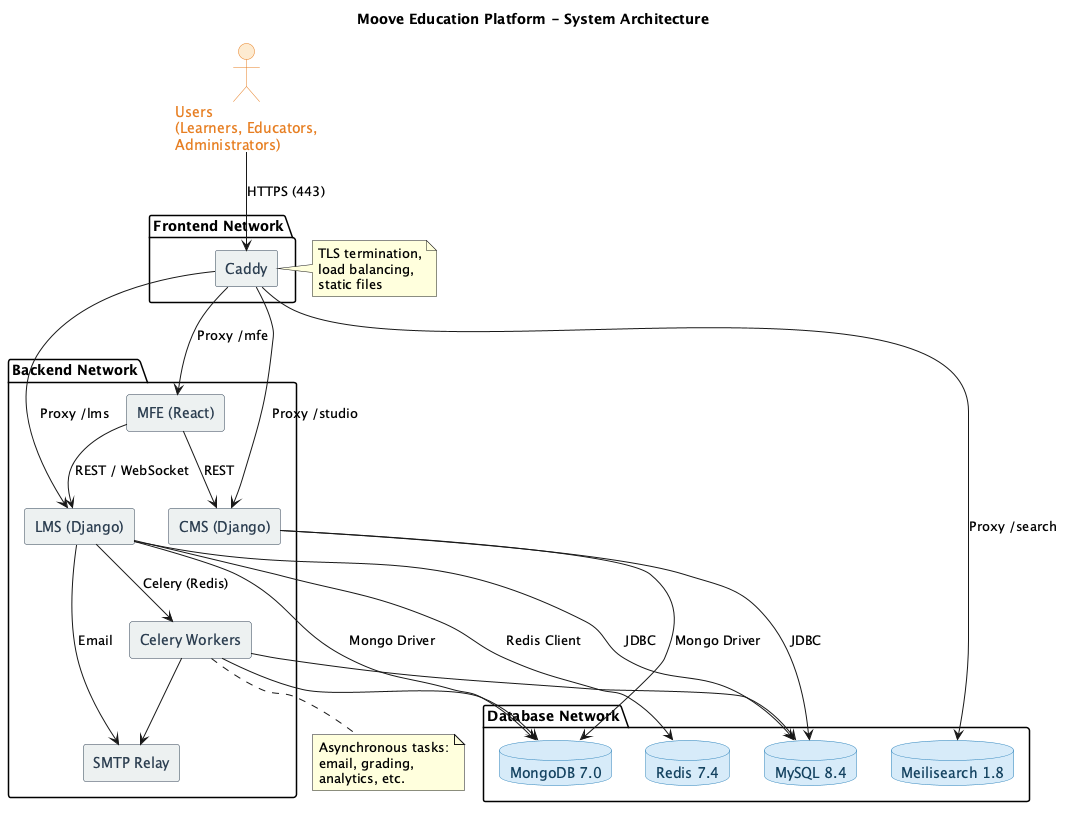
\includegraphics[width=\textwidth,height=0.7\textheight,keepaspectratio]{diagrams/system_architecture.png}
\caption{System Architecture Diagram showing Caddy, LMS, CMS, MFE, databases, and supporting services.}
\label{fig:system_arch}
\end{figure}

\subsection{Data Flow Diagram (DFD)}
The Data Flow Diagram shows how data moves through the system, from user interactions to storage and retrieval.

\subsubsection{Context Diagram (Level 0)}
\begin{figure}[H]
\centering
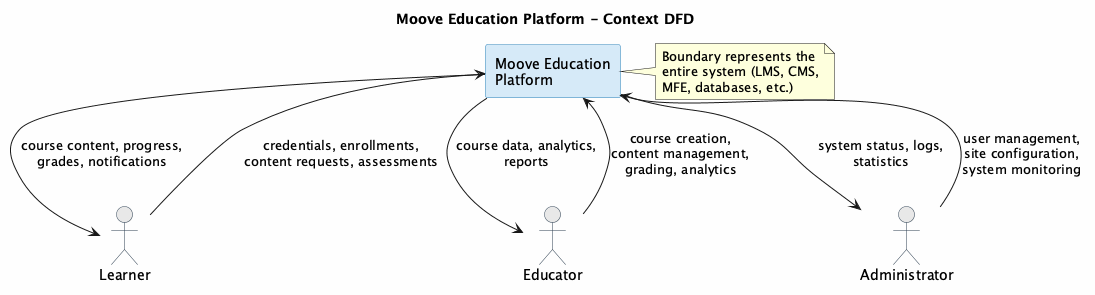
\includegraphics[width=0.8\textwidth,height=0.6\textheight,keepaspectratio]{diagrams/dfd_context.png}
\caption{Context DFD showing external entities (Learner, Educator, Administrator) and the system boundary.}
\end{figure}

\subsubsection{Level 1 DFD}
\begin{figure}[H]
\centering
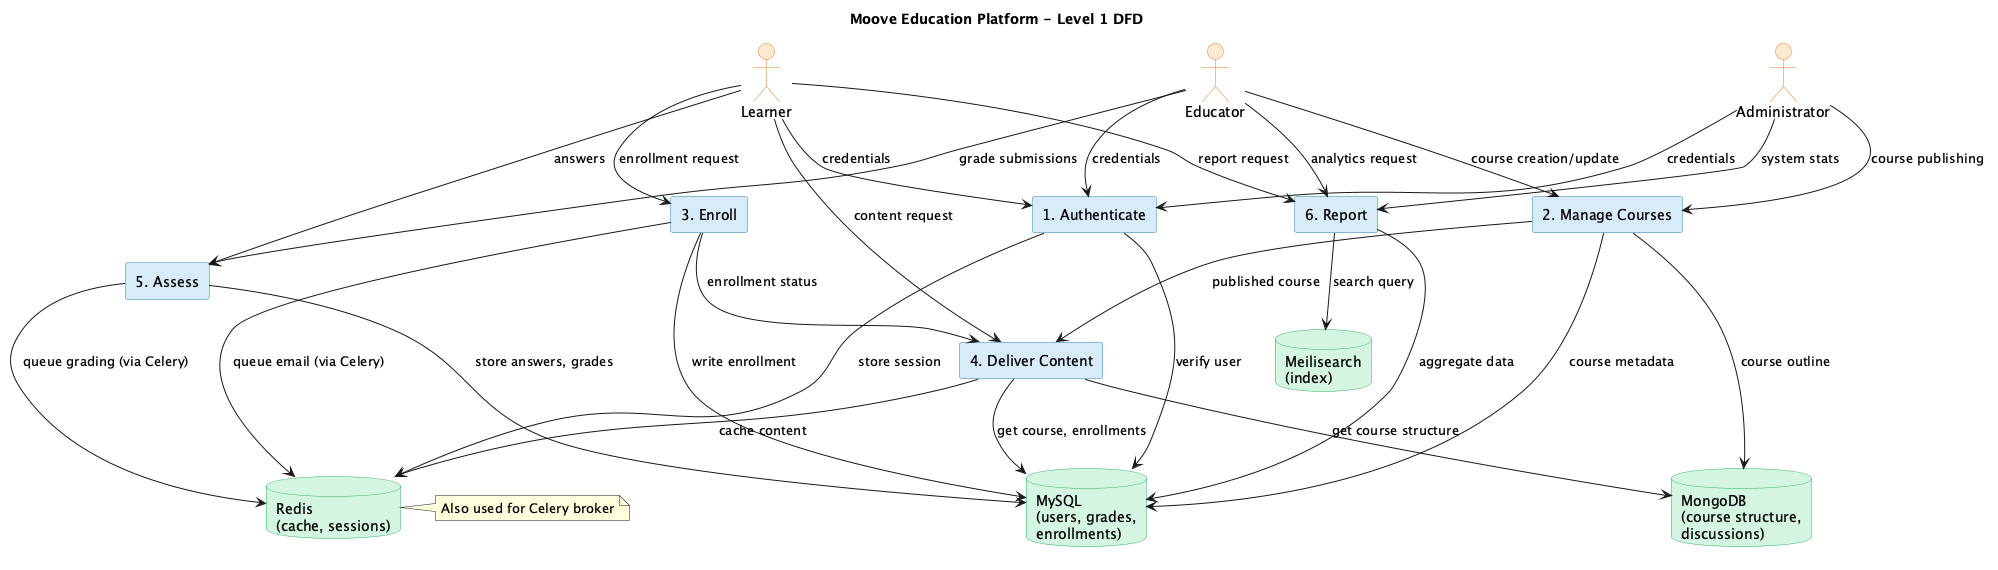
\includegraphics[width=\textwidth,height=0.7\textheight,keepaspectratio]{diagrams/dfd_level1.png}
\caption{Level 1 DFD showing main processes: Authentication, Course Management, Enrollment, Content Delivery, Assessment, and Reporting.}
\end{figure}

\subsection{Data Flow Explanation}
The system processes data as follows:

\begin{itemize}
    \item \textbf{Authentication:} User credentials are submitted via the MFE or LMS. Caddy passes the request to the LMS, which validates against MySQL and returns a session token (JWT).
    \item \textbf{Course Management:} Educators create course structures in the CMS. Data is stored in MySQL (course metadata) and MongoDB (course outline, XBlock content). When published, the LMS reads this data to render course content.
    \item \textbf{Enrollment:} When a learner enrolls, the LMS writes the enrollment record to MySQL and triggers a Celery task to send a confirmation email.
    \item \textbf{Content Delivery:} Learners request course pages; the LMS fetches the course structure from MongoDB, renders the content (using Django templates or MFE), and serves it via Caddy.
    \item \textbf{Assessments:} Learner answers are sent to the LMS, validated, and stored in MySQL. Grade calculations are performed asynchronously by Celery workers.
    \item \textbf{Search:} Meilisearch indexes course content and discussions. Search queries are routed through Caddy to the Meilisearch API.
    \item \textbf{Notifications:} The system generates notification events (e.g., discussion replies, assignment due dates) via Redis and Celery, sending emails through the SMTP relay.
\end{itemize}

\section{Security Architecture (INSA Compliance)}
This section describes the security controls implemented to meet INSA requirements. Detailed risk assessment and threat modelling are provided in the \textit{Security Architecture \& Threat Model} document.

\subsection{Network Security}
\begin{itemize}
    \item Host firewall (UFW) is enabled and configured to allow only SSH (22), HTTP (80), and HTTPS (443) from external networks.
    \item Internal container networking is segmented into three Docker networks: \texttt{frontend}, \texttt{backend}, and \texttt{database}. The database network is internal and not exposed to the host.
    \item All unnecessary ports and services are disabled.
    \item Rate limiting and brute‑force protection are provided by fail2ban.
\end{itemize}

\subsection{Container Isolation}
\begin{itemize}
    \item Each service runs in its own container with minimal privileges.
    \item Tutor runs under a dedicated non‑root user (\texttt{tutor}) with membership in the \texttt{docker} group.
    \item Resource limits (CPU, memory) are applied to containers to prevent resource exhaustion.
\end{itemize}

\subsection{Secrets Management}
\begin{itemize}
    \item All sensitive configuration values (passwords, API keys, private keys) are stored encrypted and rotated regularly.
    \item Secrets are managed via Tutor’s configuration system and not hard‑coded in source code.
    \item JWT RSA private key is stored securely and rotated periodically.
\end{itemize}

\subsection{Monitoring and Logging}
\begin{itemize}
    \item Centralised logging is implemented using the ELK stack (Elasticsearch, Logstash, Kibana).
    \item Security events (login failures, privilege changes) are logged and monitored.
    \item Weekly vulnerability scanning of container images is performed using Trivy.
\end{itemize}

\subsection{Compliance}
\begin{itemize}
    \item The architecture is designed to meet CMCSRS requirements for access control, cryptography, and incident response.
    \item Annual security audits and accreditation are planned.
    \item All security controls are documented and tested.
\end{itemize}

For a complete threat model and risk assessment, refer to the \textit{Security Architecture \& Threat Model} (Security\_OpenEdX.tex).

\section{UML Diagrams}
\subsection{Use Case Diagram}
\begin{figure}[H]
\centering
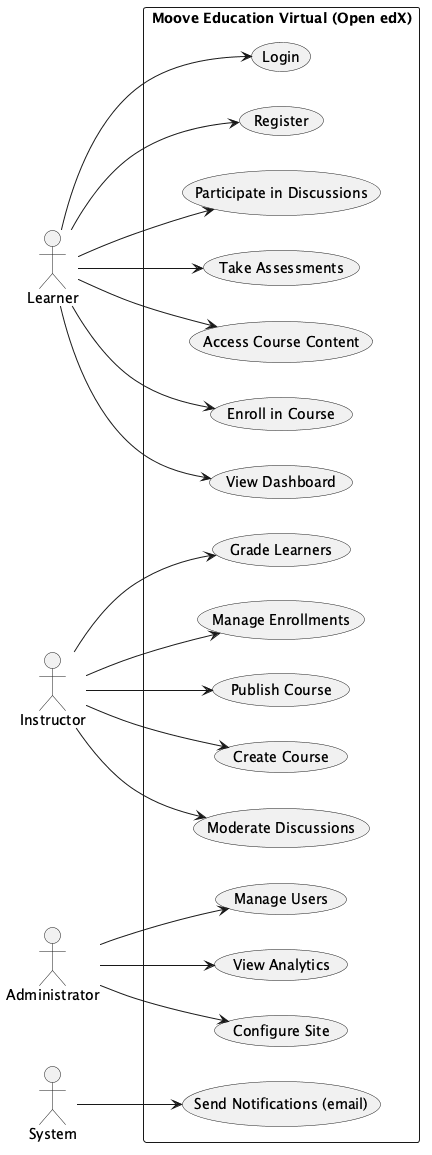
\includegraphics[width=\textwidth,height=0.7\textheight,keepaspectratio]{diagrams/usecase.png}
\caption{Use Case Diagram showing Educator and Learner interactions.}
\end{figure}

\subsection{Class Diagram}
\begin{figure}[H]
\centering
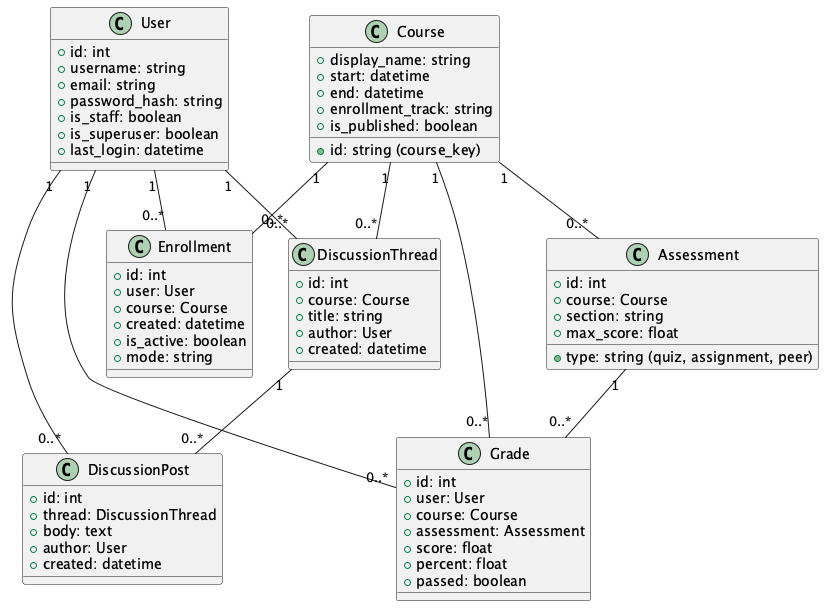
\includegraphics[width=\textwidth,height=0.7\textheight,keepaspectratio]{diagrams/class.png}
\caption{Core entities: User, Course, Enrollment, Assessment, Grade, Discussion.}
\end{figure}

\subsection{Sequence Diagram: Course Enrollment}
\begin{figure}[H]
\centering
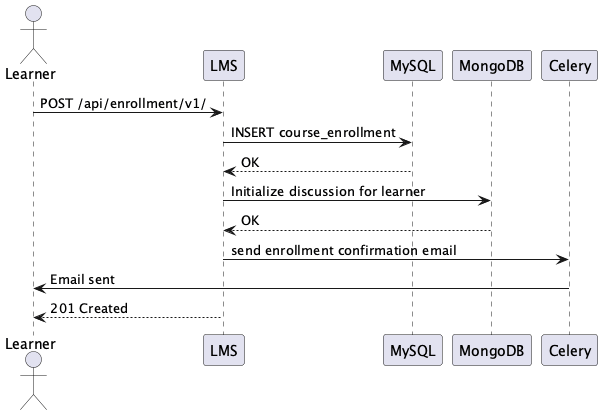
\includegraphics[width=\textwidth,height=0.7\textheight,keepaspectratio]{diagrams/sequence_enrollment.png}
\caption{Learner enrollment flow.}
\end{figure}

\subsection{Sequence Diagram: Course Creation (Educator)}
\begin{figure}[H]
\centering
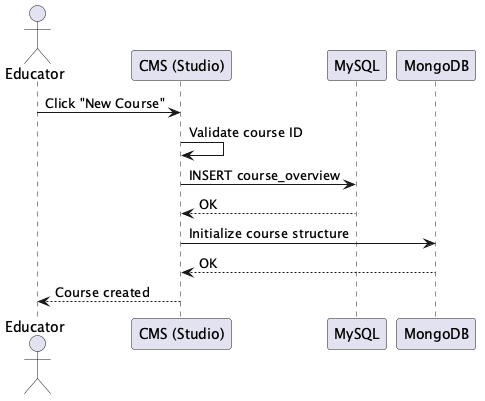
\includegraphics[width=\textwidth,height=0.7\textheight,keepaspectratio]{diagrams/sequence_course_creation.png}
\caption{Educator course creation flow.}
\end{figure}

\section{Module Interaction}
Refer to the TDD for detailed component diagrams and API interactions.

\section{References}
\begin{itemize}
    \item \textit{Security Architecture \& Threat Model – Moove Education Platform} (Security\_OpenEdX.tex)
    \item CMCSRS v2.0
    \item FDRE National Cybersecurity Policy (2024)
\end{itemize}

% === LICENSE ATTRIBUTION ===
\newpage
\section*{Apache License 2.0 Attribution}
This product includes software developed by the \textbf{Open edX Project} (\url{https://open.edx.org/}) licensed under the Apache License, Version 2.0 (\url{http://www.apache.org/licenses/LICENSE-2.0}).

\textit{Moove Education Platform is a derivative work of Open edX. No modifications have been made to the original license terms. A copy of the full license text is available in the root of the source repository and in Appendix A of this document.}

% === OPTIONAL: Include full license in appendix ===
\appendix
\section{Full Apache License 2.0 Text}
\input{../common/license}

\end{document}
\end{document}